\documentclass[aspectratio=1610,hyperref={bookmarks=false}]{beamer}
\usepackage{pgfpages}
%\setbeameroption{show notes on second screen=right}

\usepackage{prolog}
\usepackage{eurosym}
\usepackage{booktabs}

%\usepackage{media9}

\usepackage{tikz}
\usetikzlibrary{calc}
\usetikzlibrary{circuits.logic}
\usetikzlibrary{circuits.logic.US}

\usepackage{etex}
\usepackage{pgfplots}
\pgfplotsset{compat=1.10}

% align caption text; no text under 'Abbildung'
\usepackage[format=hang,justification=raggedright,compatibility=false]{caption}

\usepackage[binary-units]{siunitx}
\DeclareSIUnit[number-unit-product = {}]{\inch}{\textquotedbl}
\DeclareSIUnit[number-unit-product = {}]{\ppb}{ppb}
\sisetup{
	exponent-product = \cdot,
	per-mode=fraction,
	range-phrase = --,
	group-minimum-digits = 4,
}

\newcommand{\thetelefonnumber}{0681 842 554 90}

\begin{document}
	\titleFrame{Computer?}{Das passiert in der Hardware,\\ wenn ich einen
		Befehl eingebe.}

	\begin{frame}
	\frametitle{Fahrplan}

	\begin{block}{Was werden wir heute machen?}
		\begin{itemize}
			\item Einen Einblick in eines der wichtigsten Werkzeuge eines
				Technikers geben: die Abstraktion.
			\item Dabei anhand von Beispielen aufzeigen, dass Abstraktionen
				Grenzen haben und spannendes Verhalten verstecken kann.
			\item Einen ersten Eindruck in das Entstehen eines Computerchips
				und die dabei auftretenden Probleme geben.
		\end{itemize}
	\end{block}
\end{frame}

\begin{frame}
	\frametitle{Abstraktion --- Was ist das?}

	\begin{block}{Abstraktionen sind überall!}
		\begin{itemize}
			\item Eine Abstraktion ist ein Modell.
			\item Dieses Modell versteckt komplexes Verhalten durch Weglassen
				von Informationen/Details.
			\item Dadurch ist ein Sachverhalt leichter zu verstehen, als durch die
				Summe der zugrundeliegenden Modelle.
				% In Software: Module
				% In Hardware: Komponenten
				% Erdbeschleuigung ~9.81; jedoch 0.5% zwischen Äquator und den Polen!
			\item Abstraktionen haben aber auch ihre Grenzen!
		\end{itemize}
	\end{block}

\end{frame}

\begin{frame}
	\frametitle{Abstraktion --- Beispiel: analog vs.\ digital}

	\begin{exampleblock}{Was bedeutet logisch 1 bzw.\ logisch 0?}
		Abstraktion des gemessenen Signals

		\begin{columns}[c]
			\begin{column}{.45\textwidth}
				\begin{figure}[h]
					\centering
					\begin{tikzpicture}
						\pgfplotsset{set layers=standard}
						\pgfplotsset{width=7cm}
						\pgfplotsset{colormap={hot}{color(0cm)=(blue); color(1cm)=(red)}}
						\begin{axis}[xlabel={t},
								ylabel={Spannung},
								xminorticks=false,
								xmajorticks=false,
								yminorticks=false,
								ymajorticks=false,
								axis x line=center,
								axis y line=left,
								ymin=-.1,
								ymax=1.1,
							]
							\pgfonlayer{axis background}
								\fill[color=blue!20!white] (axis cs:0,-0.1) -| (axis cs:1,0.4) -| cycle;
								\fill[color=red!20!white] (axis cs:0,1.1) -| (axis cs:1,0.6) -| cycle;
								\node at (axis cs: .1, .9) {log.\ 1};
								\node at (axis cs: .1, .1) {log.\ 0};
							\endpgfonlayer
							\addplot[mesh, point meta=y] table {plotdata/real_step.dat};
						\end{axis}
					\end{tikzpicture}
				\end{figure}
			\end{column}
			\begin{column}{.45\textwidth}
				\begin{figure}[h]
					\centering
					\begin{tikzpicture}
						\pgfplotsset{set layers=standard}
						\pgfplotsset{width=7cm}
						\pgfplotsset{colormap={hot}{color(0cm)=(blue); color(5mm)=(black); color(1cm)=(red)}}
						\begin{axis}[xlabel={t},
								ylabel={Spannung},
								xminorticks=false,
								xmajorticks=false,
								yminorticks=false,
								ymajorticks=false,
								axis x line=center,
								axis y line=left,
								ymin=-.1,
								ymax=1.1,
							]
							\pgfonlayer{axis background}
								\fill[color=blue!20!white] (axis cs:0,-0.1) -| (axis cs:1,0.4) -| cycle;
								\fill[color=red!20!white] (axis cs:0,1.1) -| (axis cs:1,0.6) -| cycle;
								\node at (axis cs: .1, .9) {log.\ 1};
								\node at (axis cs: .1, .1) {log.\ 0};
							\endpgfonlayer
							\addplot[mesh, point meta=y, thick, line cap=round] table {plotdata/ideal_step.dat};
						\end{axis}
					\end{tikzpicture}
				\end{figure}
			\end{column}
		\end{columns}

	\end{exampleblock}
\end{frame}

\begin{frame}
	\frametitle{Abstraktion --- Beispiel: Handy}

	\begin{exampleblock}{Handy}
		Wir können damit Anrufe tätigen und vieles mehr.
		\begin{itemize}
			\item Von der Übertragung der Daten zwischen Handy und Mast
				bemerken wir nichts. Allerdings ist hier komplizierte
                                Hochfrequenztechnik im Einsatz.
			\item Die Übertragung der Sprache passiert einfach. Warum und wie
				ist beim Telefonieren eigentlich egal, oder?
			\item Wie das Handy eine Verbindung zu einem
				Gesprächsteilnehmer aufbaut ist uns als Anwender auch egal:
                                Wir wählen nur eine Nummer.
			\item Wie reagiert das Handy auf unsere Eingabe? Was
				passiert bei einem Tastendruck?
		\end{itemize}
		\uncover<2->{
			\medskip
			Wir sehen schon mehrere Abstraktionen:
			\begin{itemize}
				\item Was ist die ``übermittelte Sprache'' eigentlich genau?
				\item Wie/wovon wird das Handy gesteuert?
			\end{itemize}
		}
	\end{exampleblock}

	%\begin{exampleblock}{Ladevorgang vom Webserver}
	% jetzt könnten wir runter gehen bis auf Elektronen die sich bewegen. Doch
	% wenn wir uns beim Laden einer Website über Elektronen gedanken machen
	% müssten, würden nicht viele Leute überhaupt einen Browser bedienen
	% können.
\end{frame}



	\begin{frame}[allowframebreaks]
	\frametitle{Computer?}
	\framesubtitle{Das passiert in der Hardware, wenn ich einen Befehl
	eingebe.}

	\begin{block}{Die Frage ist doch:}
		Muss man wissen was in der Hardware passiert?
	\end{block}
	\note{
		Wissen muss man es nicht immer.
		Genau dafür gibt es die Abstraktion:
		Man muss nicht alles wissen.
		Aber: öfters ist es gut um einen Fehler zu finden, etwas selber zu
		entwerfen oder die Leistung zu steigern
	}

	\framebreak

	\begin{block}{Machen wir ein kleines Hardwareprojekt und schauen nach!}
		Dabei werden wir
		\begin{itemize}
			\item sehen dass doch viel mehr hinter einem kleinen Gadget
				steckt als man denken mag.
			\item einen ersten Eindruck gewinnen, wie ein Computer aufgebaut ist und was denn so alles
				passiert wenn man damit interagiert.
			\item uns punktuell anschauen welche Kompetenzen man im Informatikstudium, am Beispiel
				der Technischen Informatik, erwirbt.
		\end{itemize}
	\end{block}
\end{frame}

\section{Das Projekt}
\begin{frame}
	\frametitle{Projekt Handy}

	\note{
				% Die Notes sind mehr als Aussagen/Gedanken des Vortragenden zu
				% sehen.
		Es wird zwar kein Smartphone, ist aber noch immer ein Computer im
		eigentlichen Sinne.
	}

	\begin{figure}
		\centering
		\includegraphics[width=.7\textwidth]{images/phone_almost.jpg}
		\caption{Ein Handy?}
	\end{figure}

	\pause

	\begin{center}
		Was brauchen wir dafür?
	\end{center}
\end{frame}

\begin{frame}
	\frametitle{Projekt Handy --- Display}

	\begin{figure}
		\centering
		\includegraphics[height=.5\textheight]{images/pitft.jpg}
		\caption{PiTFT by Adafruit CC BY-SA 3.0}
	\end{figure}

	\vspace{-0.5cm}

	\begin{itemize}
		\item \SI{2.8}{\inch} TFT + resistiver Touchscreen.
		\item 320$\times$240 Pixel mit je 16 Bit Farbinformation.
		\item ansprechbar über SPI Interface.
	\end{itemize}
\end{frame}

\begin{frame}
	\frametitle{Projekt Handy --- Display}

	\begin{itemize}
		\item Jedes Computersystem hat in irgendeiner Form eine Interaktion mit
			dem Benutzer.
		\item Das kann im einfachsten Fall  Taster + LED sein.
		\item In unserem Fall ist ein Touchscreen im Einsatz.
	\end{itemize}
\end{frame}

\begin{frame}
	\frametitle{Projekt Handy --- Mobilfunk}
			% Wir brauchen eine Anbindung an das Mobilnetz
	\begin{figure}
		\centering
		\includegraphics[height=.55\textheight]{images/modem.jpg}
		\caption{EFCom Pro GPRS/GSM Module}
	\end{figure}
%\end{frame}

	\vspace{-0.5cm}

%\begin{frame}
%	\frametitle{Projekt Handy -- Mobilfunk}
	\begin{itemize}
		\item SIM900 Quad-Band GSM/GPRS Module.
		\item ansprechbar über serielle Schnittstelle und AT-Commands.
	\end{itemize}
\end{frame}

\begin{frame}
	\frametitle{Projekt Handy --- Mobilfunk}

	\begin{block}{Computer kommunizieren und interagieren typischerweise}
		\begin{itemize}
			\item mit dem Benutzer\\
			per ``User Interface''
			\item \emph{mit anderen Computern} \\
			``Vernetzung'', ``verteilte Systeme''
			\item mit der Umwelt\\
			 per Sensor/Aktor, ``Embedded Systems''
		\end{itemize}
	\end{block}
\end{frame}

\begin{frame}
	\frametitle{Projekt Handy --- Steuerung}
	\begin{figure}
		\centering
		\includegraphics[height=.55\textheight]{images/rpi.jpg}
		\caption{Raspberry Pi B}
	\end{figure}
%\end{frame}
\vspace{-0,5cm}
%\begin{frame}
%	\frametitle{Projekt Handy -- Steuerung}
	\begin{itemize}
		\item Broadcom BCM2835 @ \SI{700}{\mega\hertz} ARM11 core,
			\SI{256}{\mega\byte}  RAM.
		\item 26 Pin Header für Erweiterungen \ldots
		\item bietet SPI und serielle Schnittstelle.
	\end{itemize}
\end{frame}

\begin{frame}
	\frametitle{Projekt Handy --- Steuerung}

	\begin{itemize}
		\item Macht die ``Intelligenz'' im System aus.
		\item Ermöglicht die Programmierung entsprechend der Anwendung (Handy, Alarmmelder, Anrufbeantworter, \ldots).
		\item Führt passende Ansteuerung von Touchscreen und Modem durch.
		\item Macht aus der Summe der Teile ein Handy.
	\end{itemize}

\end{frame}

\begin{frame}
	\frametitle{Projekt Handy --- Energie}
	Jeder Computer braucht eine Energiequelle; \\
	in unserem Fall soll sie portabel sein.
	\begin{figure}
		\centering
		\includegraphics[height=.4\textheight]{images/akku.jpg}
		\caption{Akkupack}
	\end{figure}
	\vspace{-0.5cm}
	\begin{itemize}
		\item Akkupack mit integrierter Ladeelektronik.
		\item \SI{2200}{mAh}
	\end{itemize}
\end{frame}

\begin{frame}
	\frametitle{Projekt Handy --- Kostenaufstellung}
	\note{Kicken?}
	\begin{center}
		\begin{tabular}{rl} \toprule
			Preis (\euro) & Komponente \\ \midrule
			35 & Raspberry Pi\\
			35 & Adafruit PiTFT\\
			40 & EFCom GPRS/GSM Module\\
			15 & Akku\\
			5 & Kleinteile\\\cmidrule(lr){1-2}
			130 & Gesamt\\
			\bottomrule
		\end{tabular}
	\end{center}
\end{frame}

\liveDemo{Projekt Handy --- Putting it all together}

\begin{frame}
    \centering
	\begin{block}{Quiz:}
		Wie nennt man die kleinste Informationseinheit, die ein Computer
		verarbeitet?
		\begin{enumerate}
			\item PIN
			\item BIT
			\item LED
			\item PUK
		\end{enumerate}
	\end{block}

	\medskip

	\uncover<2->{
		\huge
		\thetelefonnumber
	}
\end{frame}

\begin{frame}
	\frametitle{Was wissen wir eigentlich über \ldots}
			% Prüfungsfach Programmierung

			% Ansteuerung des Displays und Interaktion mit dem Modem

	\begin{block}{\ldots den Rechner?}
		\begin{itemize}
			\item Ein Rechner umfasst Prozessor, Speicher und Peripherie.
			\item Der Prozessor versteht Befehle und kann daher programmiert werden.
			\item Nicht jeder Prozessor ist gleich, je nach Hersteller versteht er
				andere Befehle.
			\item Wie der Prozessor auf Hardware Ebene genau funktioniert, werden
				wir uns morgen genauer ansehen.
			\item Für unser Projekt ist uns das egal, durch die Verwendung
				einer \alert<2->{Programmiersprache} abstrahieren wir das
				alles weg und \alert<2->{arbeiten prozessorunabhängig} (soweit
				es geht).

		\end{itemize}
	\end{block}
\end{frame}

\begin{frame}
			% Abstraktion: Wie der Touch funktioniert ist egal, wir bekommen von
			% einem Treiber nur gesagt wo gedrückt wurde und reagieren darauf

	\begin{block}{\ldots den Touchscreen?}
		\begin{itemize}
			\item Wie wird der Druck des Fingers erkannt?
			\item Durch Änderung der Kapazität an einer bestimmten Koordinate
			\item oder durch einen Spannungsabfall.

			\item Aber: Wie genau, ist uns eigentlich egal (Abstraktion!).
			\item \alert<2->{Wir bekommen nur die Information wo gedrückt wurde.}
		\end{itemize}
	\end{block}
\end{frame}

\begin{frame}
	\begin{block}{\ldots das Display?}
		\begin{itemize}
			\item Wie kommt ein Zeichen auf das Display?
			\item Spannung steuert, wie ein Flüssigkristall die Polarisationsrichtung von Licht beeinflusst.
			\item \alert<2->{Wir sagen nur, was wo am Display sein soll.}
		\end{itemize}
	\end{block}
\end{frame}


\begin{frame}

	\begin{block}{\ldots das Modem?}
		\begin{itemize}
			\item Wie funktioniert eigentlich die Funkübertragung?
			\item Über kontrollierte (modulierte) elektromagnetische
				Wellenausbreitung.
			\item Wie wandelt das Modem digitale Daten in elektromagnetische
				Wellen um?
			\item Wieder abstrahieren wir diese ``Details'' weg: \alert<2->{wir
					übergeben dem Modem Daten zum Senden.}
		\end{itemize}
	\end{block}
%	Stellt eine Schnittstelle zwischen dem analogen Mobilfunk und der
%	digitalen Signalverarbeitung dar.
%	Genaue funktionsweise wird im ET-Studium vermittelt, im BTI werden nur
%	Grundlagen der Elektrotechnik gebracht.
%	Jedoch ist das Modem ein ASIC (Application Specific Integrated
%	Ciruit) die sehr wohl behandelt werden.

			% Abstraktion: zwei Kabel reichen aus um viel mehr zu steuern
			% Experimentreihe: Das Kabel
\end{frame}

\begin{frame}
			% Prüfungsfach Signale und Systeme

	\begin{block}{\ldots das Audiointerface?}
		\begin{itemize}
	%		\item Neben Datendiensten ist die Sprachtelefonie noch immer eine wichtige Funktion eines Mobiltelefons
			\item Wie kommt die Sprache eigentlich von A nach B?
			\item Ein Mikrofon wandelt die Schallwellen in ein elektrisches
				Signal um.
			\item Und wie erhalten wir aus diesem elektrischen Signal einen Datenwert, der
				weiter verarbeitet werden kann?
			\item Dazu gibt es eigene Analog/Digital Konverter, die nach
				verschiedenen Prinzipien arbeiten.
			\item Doch auch diese Details nehmen uns darunter liegende Ebenen
				(HW Module, Treiber) ab, \alert<2->{wir betrachten die Signale
				einfach als digitale Daten, die wir verarbeiten.}
		\end{itemize}
	\end{block}
	\note{
		Behandlung der Daten wird von Chip gemacht; erleichtert die Arbeit
		Aliasing Demo?
	}
\end{frame}



	\begin{frame}
	\frametitle{Der Zauber der Abstraktion}

	Wir konzentrieren uns auf das Wesentliche, lassen Details weg.

	Das erlaubt uns, effizient zu sein, den Überblick zu behalten.
	\bigskip

	\begin{quote}
		Wie produktiv wäre ein Programmierer, müsste er sich stets über den
		Verlauf der elektrischen Felder in den Transistoren der Ziel-Hardware
		Gedanken machen?
	\end{quote}

	\bigskip
	Wir konnten mit fertigen Komponenten und deren abstrakter
	Funktionsbeschreibung immerhin ein ganzes Handy zusammenbauen!

\end{frame}

\sectionFrame{Wozu also ein Studium?}{Abstraktes verstehen!}

\begin{frame}
	\frametitle{Wie kommt meine Stimme ins Telefon?}
	\begin{block}{Das Audiointerface liefert digitale Daten}
		\begin{itemize}
			\item Was steht eigentlich hinter dieser Abstraktion?
			\item Gibt es da auch Grenzen und Probleme?
			\item Sollte man da auch mehr wissen?
		\end{itemize}
	\end{block}
\end{frame}

\begin{frame}[t]
	\frametitle{Digitalisieren eines Audiosignals}
	\begin{center}
		% Sinus, zuerst horizontale Linien als grid einblenden (ADC steps),
		% dann horiz Linien weg, dafür vertikale (time samples), ca 25 pro
		% Periode
		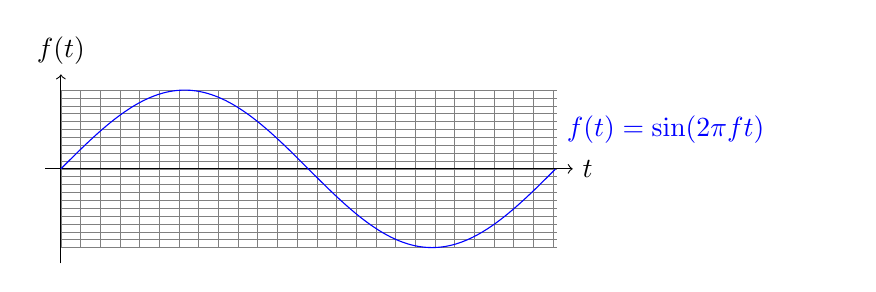
\begin{tikzpicture}[domain=0:6.28, samples=85,smooth]
			% Grundgrid
			%\draw<1>[style=help lines] (-0.1,-1.1) grid[xstep=1] (6.3,1.1);

			% 'ADC' Values
			\foreach \y in {-1,-0.9,...,1.1} { \draw<2>[style=help lines] (0,\y) -- (6.3,\y); }

			% Timesteps
			\foreach \x in {0,0.25,...,6.3} { \draw<3>[style=help lines] (\x,-1) -- (\x,1); }

			% Achsen
			\draw[->] (-0.2,0) -- (6.5,0) node[right] {$t$};
			\draw[->] (0,-1.2) -- (0,1.2) node[above] {$f(t)$};

			% Sinus
			\draw[color=blue] plot (\x,{sin(\x r)});
			\node[anchor=west,color=blue] (s1) at (6.3,0.5) {$f(t) = \sin (2 \pi f t)$};

			% Damit der Plot nicht rutscht
			\path (0,0) -- (10,0);
		\end{tikzpicture}
	\end{center}

	\begin{block}{Um das Signal digital zu verarbeiten, müssen wir}
		\begin{itemize}
			\item Amplitude
			\item und Zeit diskretisieren (``Abtastpunkte'' statt Verlauf)
		\end{itemize}
		Wie viele Abtastpunkte ($\Rightarrow$Speicherplatz) brauchen wir?
	\end{block}
\end{frame}

\begin{frame}[t]
	\frametitle{Ein Signal abtasten}
	\begin{center}
		% Sinus mit nur (etwas mehr als) 2 Samples/per einzeln einblenden:
		% höherfrequente Sinussignale die auch passen
		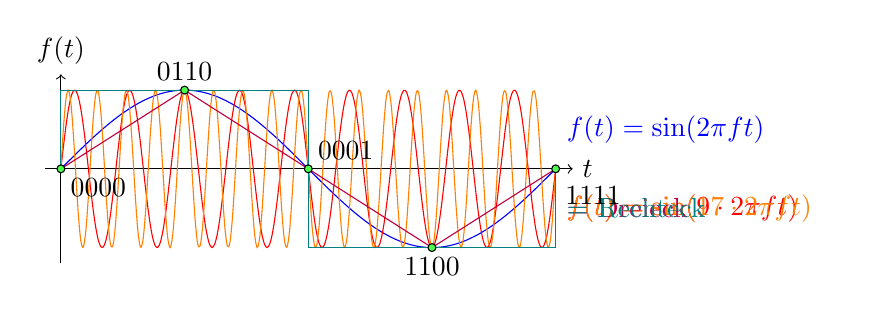
\begin{tikzpicture}[domain=0:6.28, samples=200,smooth]
			\tikzstyle{spt}=[color=black,fill=green!70]
			% Grid
%			\draw[style=help lines] (-0.1,-1.1) grid (6.3,1.1);

			% Achsen
			\draw[->] (-0.2,0) -- (6.5,0) node[right] {$t$};
			\draw[->] (0,-1.2) -- (0,1.2) node[above] {$f(t)$};

			% Grundsinus
			\draw[color=blue] plot (\x,{sin(\x r)});
			\node[anchor=west,color=blue] (s1) at (6.3,0.5) {$f(t) = \sin (2 \pi f t)$};

			% Vielfach-Sinuse
			%\draw[color=red] plot[id=v1\thecnt] (\x,{sin((#1) * (\x r) + (#2))}) node[below right]
			%	{$f(x) = \sin (#1 x)$};
			\draw<2>[color=red] plot (\x,{sin((9 * \x) r)});
			\node<2>[anchor=west,color=red] (s2) at (6.3,-0.5) {$f(t) = \sin (9 \cdot 2 \pi f t)$};

			\draw<3>[color=orange] plot (\x,{sin((17 * \x) r)});
			\node<3>[anchor=west,color=orange] (s3) at (6.3,-0.5) {$f(t) = \sin (17 \cdot 2 \pi f t)$};
			% Damit der Plot nicht rutscht
			\path (0,0) -- (10,0);

			\draw<4>[color=purple] (0,0) -- (pi/2,1) -- (pi,0) -- (3*pi/2,-1)
				-- (2*pi,0);
			\node<4>[anchor=west,color=purple] (t1) at (6.3,-0.5) {$=$ Dreieck};

			\draw<5>[color=teal] (0,0) -- (0,1) -- (pi,1) -- (pi, -1)
				-- (2*pi,-1) -- (2*pi,0);
			\node<5>[anchor=west,color=teal] (r1) at (6.3,-0.5) {$=$ Rechteck};

			% Abtastpunkte
			\draw[spt] (0,0) circle (0.05);
			\node<1>[anchor=north west] (ap1) at (0,0) {0000};

			\draw[spt] (pi/2,1) circle (0.05);
			\node<1>[anchor=south] (ap2) at (pi/2,1) {0110};

			\draw[spt] (pi,0) circle (0.05);
			\node<1>[anchor=south west] (ap3) at (pi,0) {0001};

			\draw[spt] (3*pi/2,-1) circle (0.05);
			\node<1>[anchor=north] (ap4) at (3*pi/2,-1) {1100};
			\path (3*pi/2,-1) -- +(0,-0.54);

			\draw[spt] (2*pi,0) circle (0.05);
			\node<1>[anchor=north west] (ap5) at (2*pi,-0.1) {1111};
		\end{tikzpicture}
	\end{center}

		\begin{block}{Kann ein Signal eindeutig rekonstruiert werden?}
			\uncover<2->{
				Es gibt unendlich viele Möglichkeiten ein abgetastetes Signal
				(falsch) zu rekonstruieren!
			}
		\end{block}
\end{frame}

\begin{frame}[t]
	\begin{center}
		% Robert's Signal aus 2 Sinussen: enmal als Summe, darunter die
		% einzelnen Komponenten, noch keine Abtastpunkte

		% Robert's Signal, diesmal mit zu wenigen Punkten
		%einblenden: passended niederfrequentes Signal
		%einblenden: mehr Punkte
		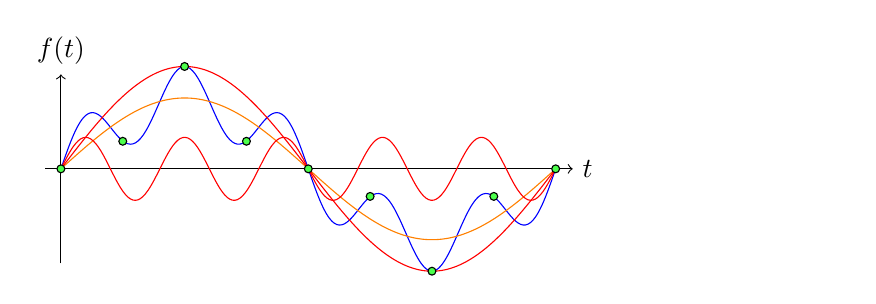
\begin{tikzpicture}[domain=0:6.28, samples=200,smooth]
			\tikzstyle{spt}=[color=black,fill=green!70]
			% Grid
%			\draw[style=help lines] (-0.1,-1.1) grid (6.3,1.1);

			% Achsen
			\draw[->] (-0.2,0) -- (6.5,0) node[right] {$t$};
			\draw[->] (0,-1.2) -- (0,1.2) node[above] {$f(t)$};

			% Überlagerung
			\draw[color=blue] plot (\x,{0.9 * sin(\x r) + 0.4 * sin((5 * \x) r)});

			% Grundsinus
			\draw<2>[color=orange] plot (\x,{0.9 * sin(\x r)});

			% Vielfach-Sinuse
			\draw<2>[color=red] plot (\x,{0.4 * sin((5 * \x) r)});

			% Simpler Match -- Nein, ich konstruiere mir meine Beispiele nicht
			% so einfach ;)
			\draw<4>[color=red] plot (\x, {1.3 * sin(\x r)});

			% Abtastpunkte
			\draw<3->[spt] (0,0) circle (0.05);
			\draw<3->[spt] (pi/2,1.3) circle (0.05);
			\draw<3->[spt] (pi,0) circle (0.05);
			\draw<3->[spt] (3*pi/2,-1.3) circle (0.05);
			\draw<3->[spt] (2*pi,0) circle (0.05);

			\draw<5->[spt] (pi/4  , 0.35) circle (0.05);
			\draw<5->[spt] (3*pi/4, 0.35) circle (0.05);
			\draw<5->[spt] (5*pi/4,-0.35) circle (0.05);
			\draw<5->[spt] (7*pi/4,-0.35) circle (0.05);

			% Damit der Plot nicht rutscht
			\path (0,0) -- (10,0);
			\path (0,0) -- (0,-1.36);

		\end{tikzpicture}
	\end{center}

	\only<2>{
		\begin{block}{Fourieranalyse:}
			\begin{itemize}
				\item Man kann jedes Signal als Summe von Sinussignalen
					darstellen.
			\end{itemize}
		\end{block}
	}
	\only<3-4>{
		\begin{block}{Wie viele Abtastpunkte brauchen wir mindestens?}
			\uncover<4->{
				Abtasttheorem: Wir brauchen zumindest 2 Abtastwerte pro
				Periode des höchstfrequenten Sinus.
			}
		\end{block}
	}
	\only<5>{
		\begin{block}{Vorgangsweise}
			\begin{itemize}
				\item Wir legen die höchste relevante Frequenz fest
					(Hörbereich \ldots).
				\item Wir filtern alle höheren Frequenzen weg (Tiefpass):\\
					Dadurch können wir bei der Rekonstruktion alle höheren
					Frequenzen ausschließen.
			\end{itemize}
		\end{block}
	}
\end{frame}

\begin{frame}
	\frametitle{Grenzen der Abstraktion}

	\begin{block}{Warum also Hintergründe verstehen, ``unter die Haube
			blicken''?}
		\begin{itemize}
			\item Interesse / Neugier?
			\item Um es ein bisschen besser machen zu können?
		\end{itemize}
	\end{block}

	\medskip

	\uncover<2->{
\begin{itemize}			
	\item Weil es auch jemanden geben muss, der die Abstraktion erstellt.
	\item	\alert<3>{Weil man Abstraktionen nur verwenden sollte, wenn man auch ihre
			Grenzen kennt!}
\end{itemize}
	}
	\medskip

	\begin{block}{Aber:}<4->
		Trifft man denn wirklich auf so komplizierte Spezialfälle wo
		Abstraktionen versagen?
	\end{block}
\end{frame}


\begin{frame}
	\frametitle{Abtasttheorem --- Ein praktisches Beispiel}

	\begin{block}{Der einsame Hirte}

		hat bei einer Spielzeit von 4:25 in unkomprimierter Form bei

		\begin{itemize}
			%Hörbeispiel; perfekter Kland
			\item<1-> Abtastung mit \SI{44100}{\hertz}: \SI{41}{\mega\byte}
				%shepherd
	%			\only<1>{
	%				\includemedia[
	%					addresource=media/shepherd_cut.mp3,
	%					flashvars={
	%						source=media/shepherd_cut.mp3&autoPlay=true
	%					}
	%				]{\fbox{Play}}{APlayer.swf}
	%			}
			%Hörbeispiel; akzeptabler Klang
			\item<2-> Abtastung mit \SI{22050}{\hertz}: \SI{21}{\mega\byte}
				%shepherd_filter_22050
	%			\only<2>{
	%				\includemedia[
	%					addresource=media/shepherd_filter_22050.mp3,
	%					flashvars={
	%						source=media/shepherd_filter_22050.mp3&autoPlay=true
	%					}
	%				]{\fbox{Play}}{APlayer.swf}
	%			}
			%Hörbeispiel; kacke Klang; fehlende Frequenzen
			\item<3-> Abtastung mit \phantom{2}\SI{2205}{\hertz}: \phantom{2}\SI{2.1}{\mega\byte}
				%shepherd_filter_2205
	%			\only<3>{
	%				\includemedia[
	%					addresource=media/shepherd_filter_2205.mp3,
	%					flashvars={
	%						source=media/shepherd_filter_2205.mp3&autoPlay=true
	%					}
	%				]{\fbox{Play}}{APlayer.swf}
	%			}
			%Hörbeispiel; kacke Klang; aliasing
			\item<4-> Abtastung mit \phantom{2}\SI{2205}{\hertz} ohne Filter: \SI{2.1}{\mega\byte}
				%shepherd_alias_2205
	%			\only<4>{
	%				\includemedia[
	%					addresource=media/shepherd_alias_2205.mp3,
	%					flashvars={
	%						source=media/shepherd_alias_2205.mp3&autoPlay=true
	%					}
	%				]{\fbox{Play}}{APlayer.swf}
	%			}

		\end{itemize}
	\end{block}

	\medskip

	\begin{block}{Die Abtastfrequenz macht's aus!}<5>
		Auch hier macht es Sinn die Theorie zu kennen!
	\end{block}
\end{frame}



	\include{kabel}


	\begin{frame}
	\frametitle{Was steckt hinter der Abstraktion ``Computer''?}

	\begin{itemize}
		\item Das ist natürlich etwas umfangreicher,
		\item daher werden wir uns morgen damit ausführlich beschäftigen.
		\item Aber jetzt wir wollen uns einmal ansehen, \ldots
	\end{itemize}

\end{frame}


\sectionFrame{
%Vom Sandkorn zum Chip\\
%oder:\\
 Woraus besteht eigentlich\\
 ein Computerchip?}{}

\begin{frame}
	\frametitle{``All computers are just carefully organized sand''}
	\begin{figure}
		\centering
		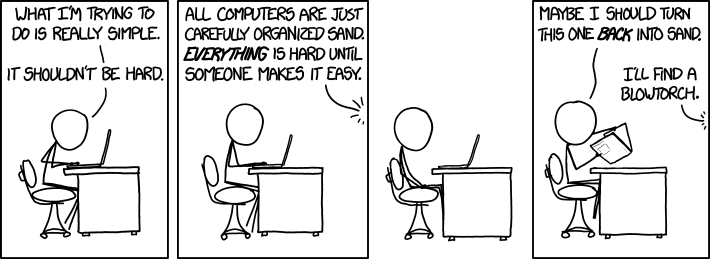
\includegraphics[width=.8\textwidth]{images/shouldnt_be_hard.png}
		\caption{``Shouldn't Be Hard'' by Randall Munroe
		CC-BY-NC-2.5, \url{http://xkcd.com/1349}}
	\end{figure}

	\begin{quote}<2->
		(six hours later) ARGH. How are these stupid microchips so durable?!
		All I want is to undo a massive industrial process with household
		tools!
	\end{quote}
\end{frame}

\begin{frame}
	\frametitle{``All computers are just carefully organized sand''}

	\begin{figure}
		\centering
		
\includegraphics[width=.7\textwidth]{images/the_desert.jpg}
		\caption{``Siliziumquelle'' SiO\textsubscript{2} \\
		``The Desert'' by John O'Nolan
		CC-BY-2.0, \url{http://flic.kr/p/aEJ8Rk}}
	\end{figure}
\end{frame}

\begin{frame}
	\frametitle{Vom Sandkorn zum Chip}
	\begin{columns}[onlytextwidth]
		\begin{column}{0.6\textwidth}
			\begin{figure}
				\centering
				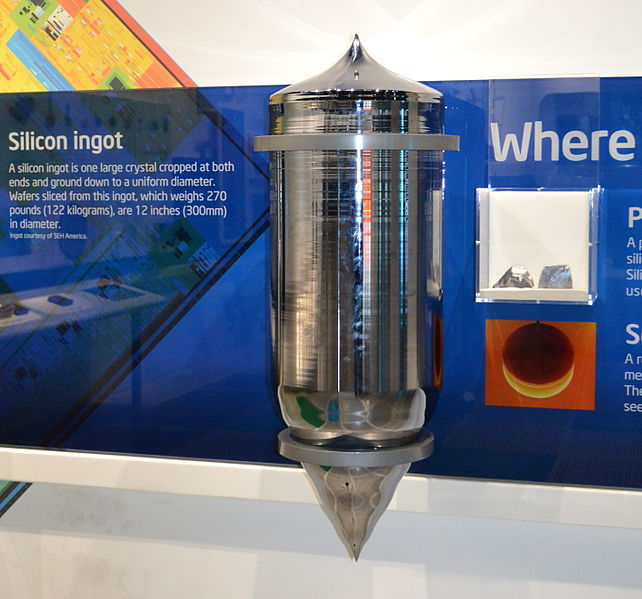
\includegraphics[width=.6\textwidth]{images/Siligon_ingot_at_Intel_Museum.JPG}

				\caption{Hochreiner Silizium-Einkristall.\\
					By Oleg Alexandrov CC-BY-SA-3.0\\
					via Wikimedia Commons.}
			\end{figure}
		\end{column}
		\begin{column}{0.45\textwidth}
			\begin{itemize}
				\item Durchmesser 30--\SI{40}{\centi\meter}
				\item Länge \SI{2}{\meter}
				\item Gewicht \SI{> 100}{\kilo\gram}
				\item Reinheitsgrad \SI{>99.9999999}{\percent}
			\end{itemize}
		\end{column}
	\end{columns}
\end{frame}

\begin{frame}
	\begin{columns}
		\begin{column}{.5\textwidth}
			\begin{figure}
				\centering
				\includegraphics[width=.85\textwidth]{images/Wafer_intel.jpg}
				\caption{Ein Wafer \textcopyright{} Intel}
			\end{figure}
		\end{column}
		\begin{column}{.5\textwidth}
			\begin{figure}
				\centering
				\includegraphics[width=.9\textwidth]{images/TTPchip.png}
				\caption{Chip im Package}
			\end{figure}
		\end{column}
	\end{columns}
\end{frame}

\begin{frame}
% good slides from intel at http://download.intel.com/newsroom/kits/chipmaking/pdfs/Sand-to-Silicon_32nm-Version.pdf
	\begin{figure}
		\centering
		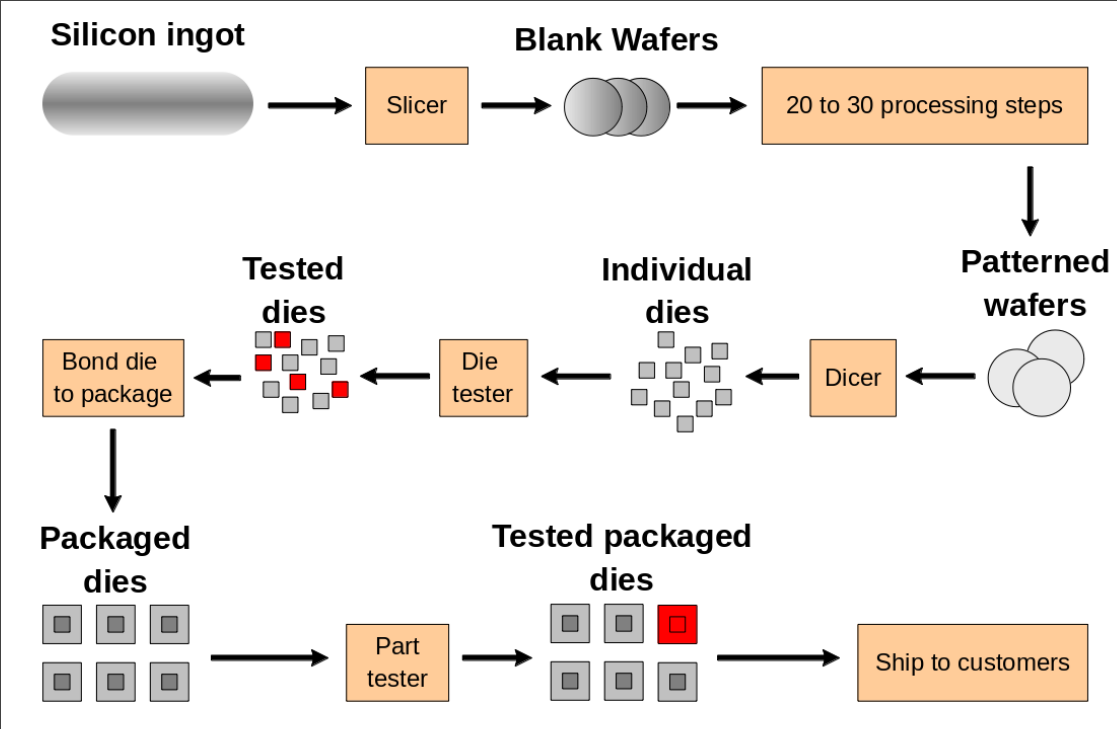
\includegraphics[width=.8\textwidth]{images/chip_fertigung.png}
		\vspace{0.3cm}
		\caption{Industrielle Chipfertigung}
	\end{figure}

\end{frame}


\begin{frame}
	\frametitle{Vom Transistor zum Mikroprozessor}
	\begin{block}{Was macht man nun mit den ganzen Transistoren?}
		\begin{itemize}
			\item Standard Cell Designer entwerfen logische Grundbausteine
				(AND, OR, NAND, \ldots) aus Transistoren in konkreter
				Technologie, z.B.\ \SI{14}{\nano\meter}.
			\item Bibliothek von solchen ``Standard Cells'' mit
				unterschiedlichen Vor-/Nachteilen: Geschwindigkeit, Größe,
				Stromverbrauch, \ldots
		\end{itemize}
	\end{block}
\end{frame}

\begin{frame}
	\begin{block}{Was macht man mit den Standard Cells?}
		\begin{itemize}
			\item Designer benutzen Standard Cell Bibliothek um Funktionsblock
				nach ihren Vorstellungen zu realisieren.
			\item Hier gibt es viel Tool-Support.
			\item Schaltungsdesigner arbeiten meist mit ``Beschreibungssprachen'',
                              ähnlich wie Programmierer.
			\item Ein komplexer Chip kann hunderte Millionen Transistoren
				beinhalten.
		\end{itemize}
	\end{block}
\end{frame}

\sectionFrame{Grenzen der Chiptechnologie}{}


\begin{frame}
	\frametitle{Chiptechnologie --- ein Größenvergleich}
	\begin{exampleblock}{Stellen Sie sich vor:}
		Ein \SI{14}{\nano\meter} Transistor % 0.058um^2
		wäre so groß wie ein Fingernagel % ~ 1 cm^2 = 10^8 um^2
                % wäre so groß wie eine Hand % 0.054 m^2 = 5.4*10^10 um^2
		\ldots\\

		\pause

		\bigskip
		\ldots dann wäre ein menschliches Haar % d ~ 100um => A ~ 7854 um^2
                so dick dass es auf dem Podium keinen Platz mehr hätte. % d ~ 3m => A < 13.36 m^2

	\end{exampleblock}

\end{frame}

\begin{frame}
	\frametitle{Chiptechnologie --- ein Größenvergleich}
	\begin{exampleblock}{Anders gesagt:}
		Ein rotes Blutkörperchen ist etwa 500x größer als ein \SI{14}{\nano\meter} Transistor!

		% kleinste RBK  d ~ 6 um => A ~ 28.27 um^2
	\end{exampleblock}
\end{frame}

\begin{frame}
	\frametitle{Chiptechnologie --- ein Generationenvergleich}
	\begin{columns}[t]
		\begin{column}{.45\textwidth}
			\begin{block}{Intel 4004}
				\begin{itemize}
					\item Einführung 1971
					\item 4-Bit (vier!) Architektur
					\item 1 Kern
					\item \SI{740}{\kilo\hertz}
					\item 2300 Transistoren
					\item 16 Pins
					\item \SI{144}{\milli\meter\squared} Die Fläche
					\item \SI{10}{\micro\meter} Prozess
				\end{itemize}
			\end{block}
		\end{column}
		\begin{column}{.55\textwidth}
			\begin{block}{Intel Core i7 4770 (Haswell)}
				\begin{itemize}
					\item Einführung 2013
					\item 64-Bit Architektur
					\item 4 Kerne
					\item \SI{3.4}{\giga\hertz}
					\item 1.4 Milliarden Transistoren
					\item 1150 Pins
					\item \SI{177}{\milli\meter\squared} Die Fläche
					\item \SI{22}{\nano\meter} Prozess
				\end{itemize}
			\end{block}
		\end{column}
	\end{columns}
\end{frame}

\begin{frame}
	\frametitle{Chiptechnologie --- ein Generationenvergleich}
	\only<1>{
		\begin{figure}
			\centering
			\includegraphics[width=.4\textwidth]{images/chip_4004-i7_then.png}
			\vspace{0.5cm}
			\caption{Die Designs in ihrer Technologie gefertigt \textcopyright{} Intel}
		\end{figure}
	}
	\only<2-3>{
		\begin{figure}
			\centering
			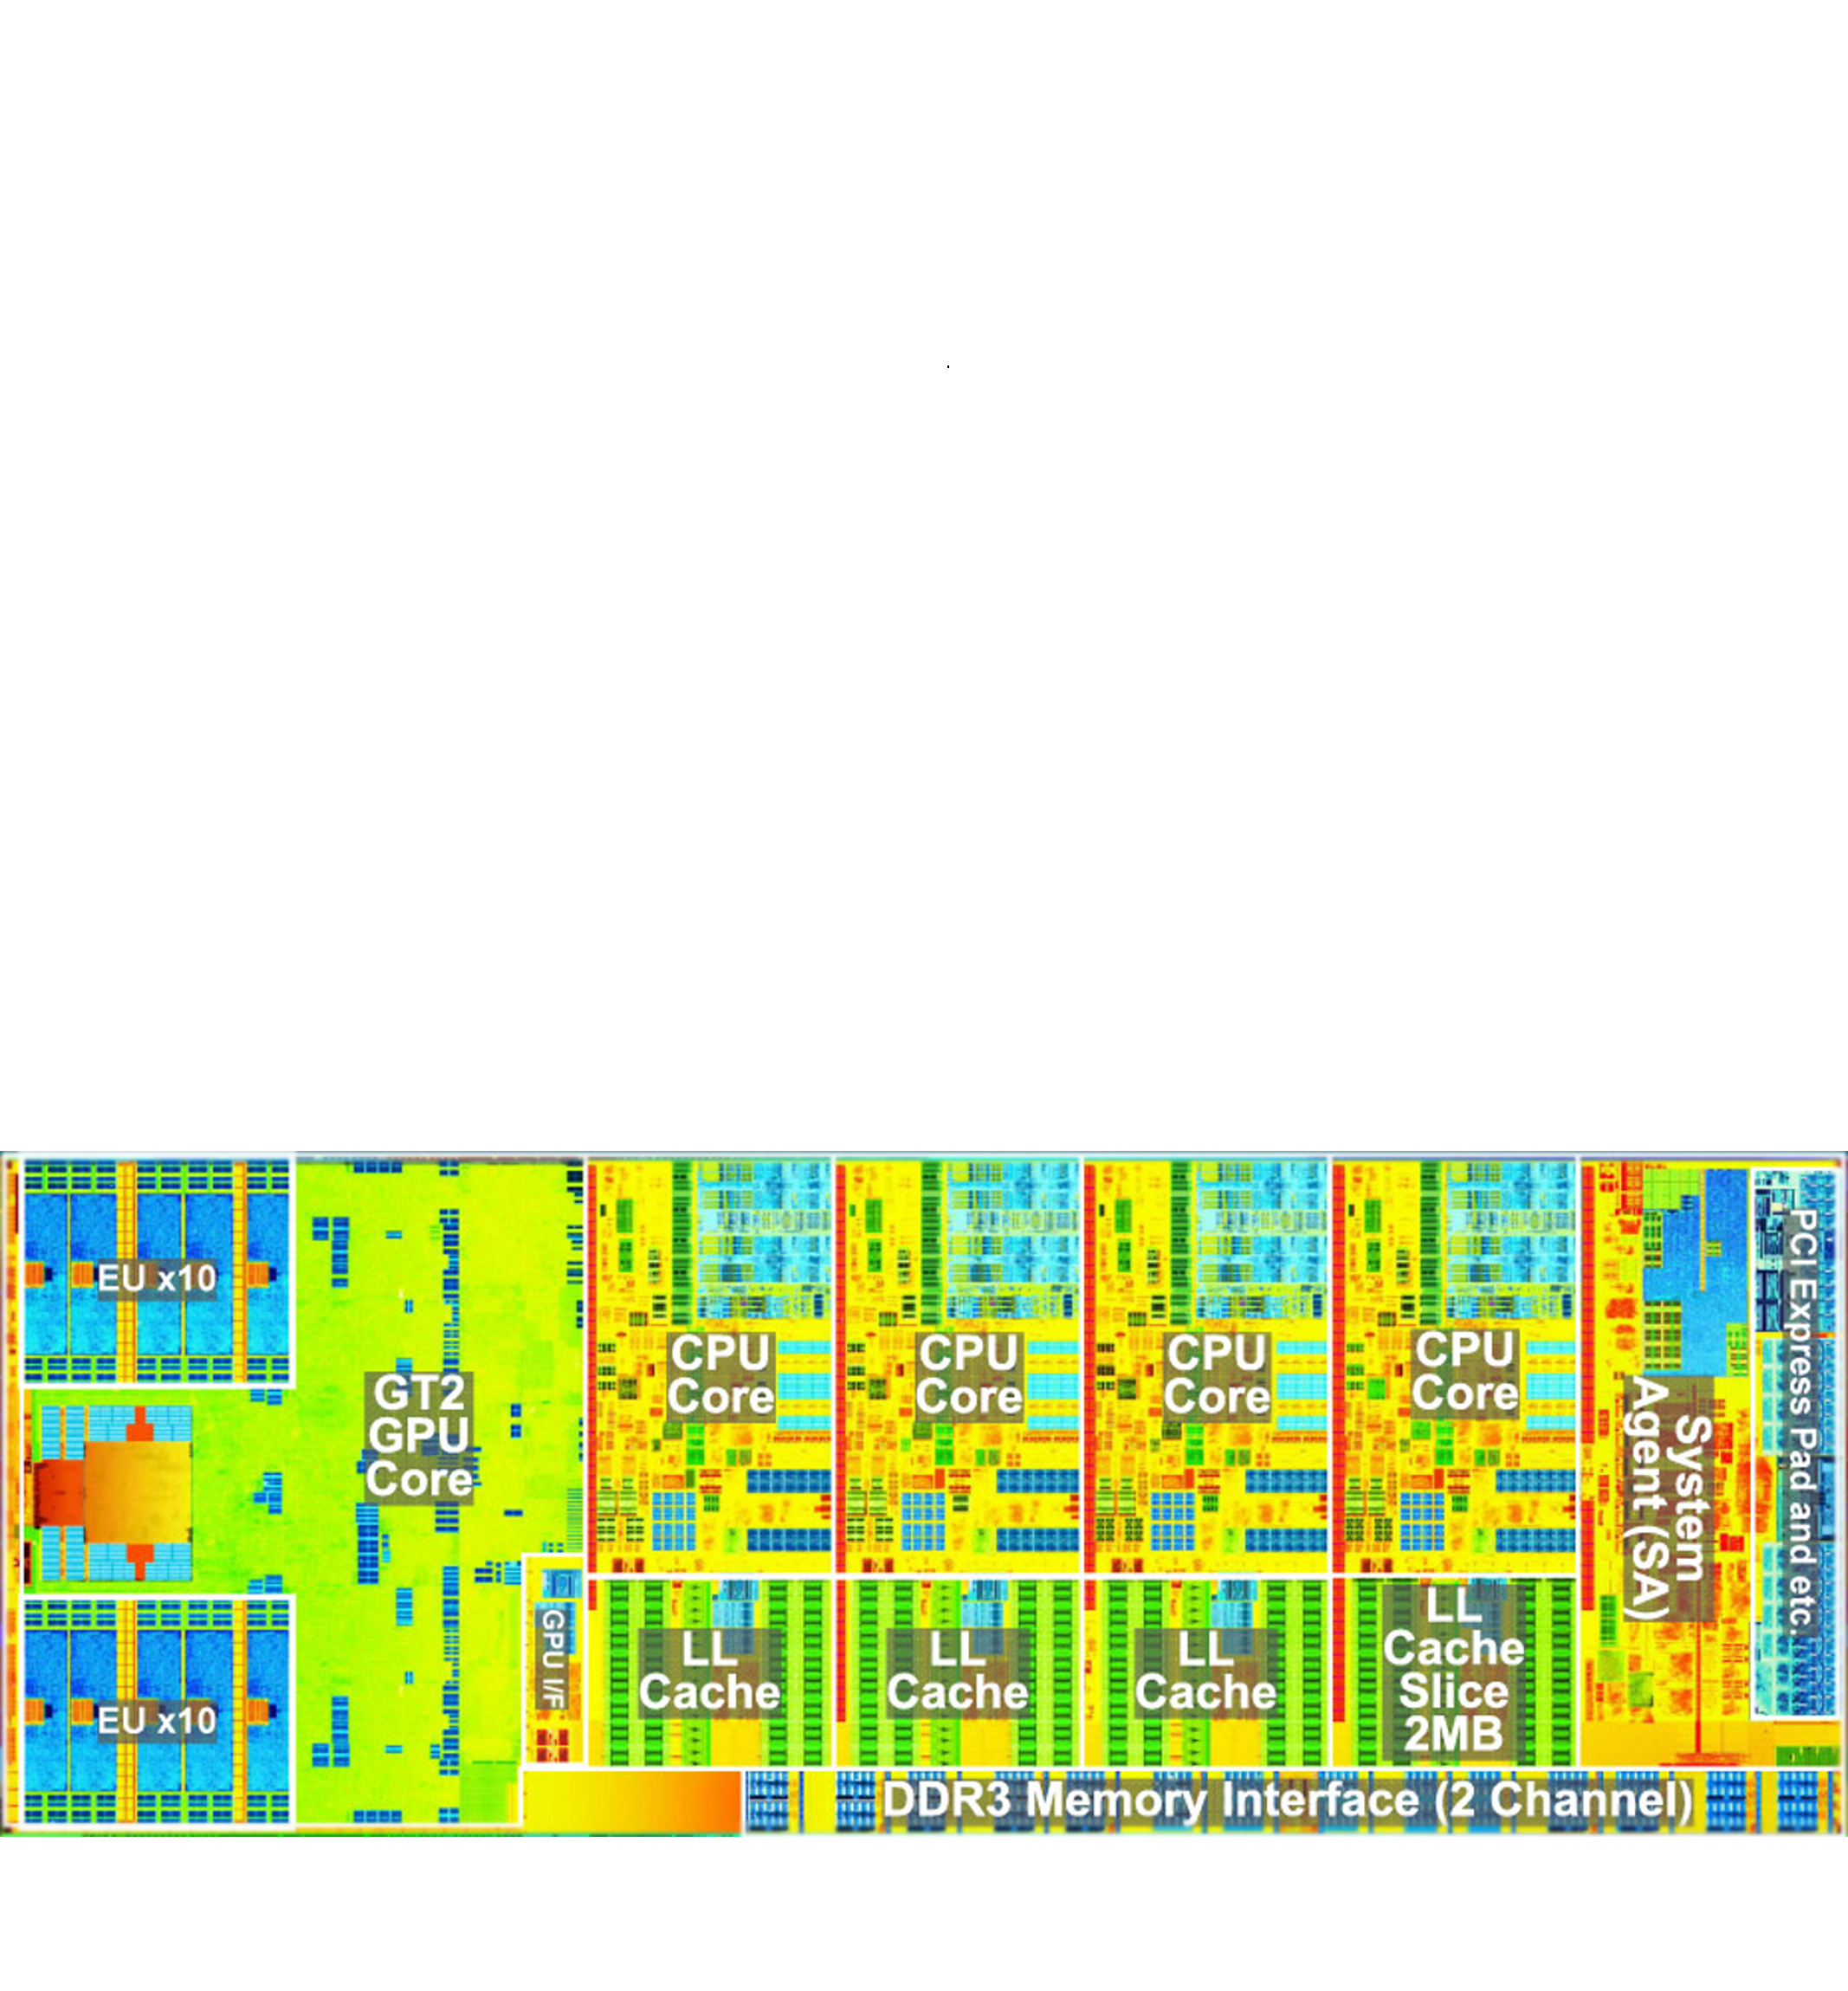
\includegraphics[width=.4\textwidth]{images/chip_4004-i7_now.png}
			\vspace{0.5cm}
			\caption{Das 40 Jahre altes Design in aktueller Technologie
				gefertigt \textcopyright{} Intel}
		\end{figure}
	}
	\begin{tikzpicture}[overlay,remember picture]
		\node[right] (i7)   at (0.7,3.7) {2013: Intel i7};
		\node<1>[below right] (four) at (0.7,7.15) {1971: Intel 4004};
		\node<2-3>[below right,align=left] (four2_2) at (0.7,7.15) {\alert{2013}: Intel 4004\\
			\SI{144}{\milli\meter\squared} $\Rightarrow$ \SI{0.0003}{\milli\meter\squared}};
		\draw<3>[latex-, red] (7.1,6.925) -- +(0.75,0.75);
	\end{tikzpicture}
\end{frame}

\begin{frame}
	\frametitle{Chiptechnologie --- Miniaturisierung}
	\only<1>{
		\begin{figure}
			\centering
			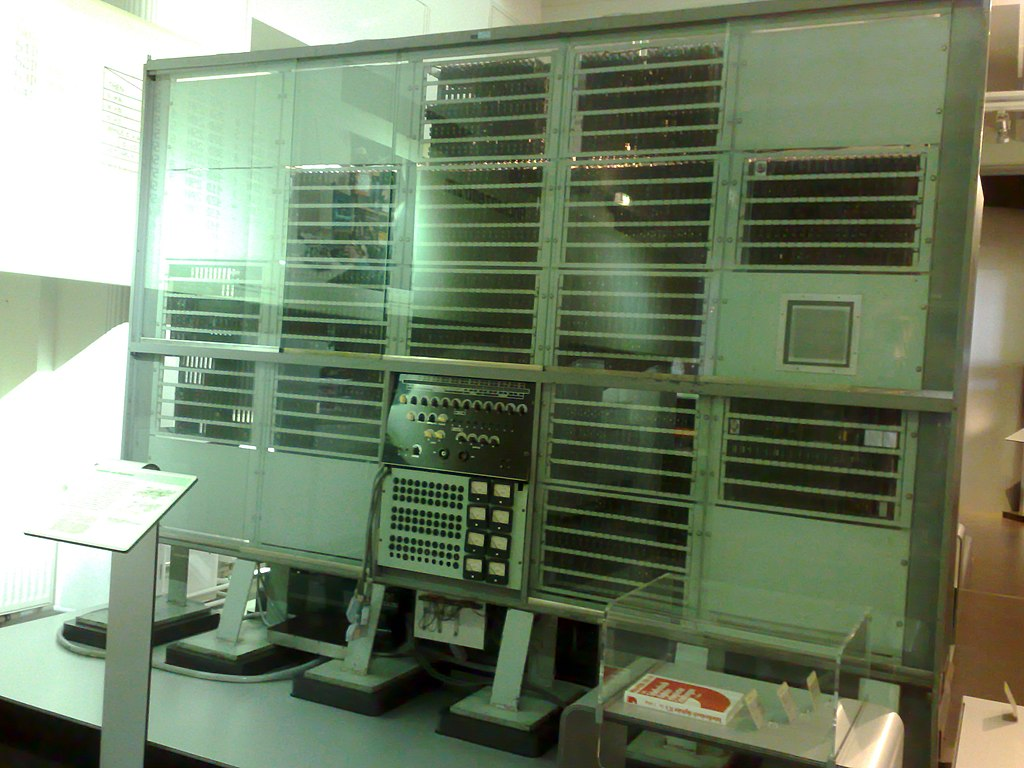
\includegraphics[height=.7\textheight]{images/Mailuefterl.jpg}
			\caption{Mailüfterl (1958); 8000 ``Transistoren'',
				\SI{20}{\kilo\meter} Schaltdraht\\
				By Florian Staudacher CC-BY-3.0 via Wikimedia Commons.}
		\end{figure}
	}
	\only<2>{
		\begin{figure}
			\centering
			\includegraphics[height=.7\textheight]{images/trans_trad.png}
			\caption{Traditionalles FET-Transistordesign \textcopyright{} Intel}
		\end{figure}
	}
	\only<3>{
		\begin{figure}
			\centering
			\includegraphics[height=.7\textheight]{images/trans_14nm.png}
			\caption{\SI{14}{\nano\meter} FinFET-Transistordesign \textcopyright{} Intel}
		\end{figure}
	}
	\only<4>{
		\begin{figure}
			\centering
			\includegraphics[height=.7\textheight]{images/14nm_fin.png}
			\caption{\SI{14}{\nano\meter} FinFET-Transistor Querschnitt \textcopyright{} Intel}
		\end{figure}
	}
	\only<5>{
		\begin{figure}
			\centering
			\includegraphics[height=.7\textheight]{images/14nm_full.png}
			\caption{\SI{14}{\nano\meter} FinFET-Transistor Querschnitt \textcopyright{} Intel}
		\end{figure}
	}
	\only<6>{
		\begin{figure}
			\centering
			\includegraphics[height=.7\textheight]{images/14nm_die.png}
			\caption{\SI{14}{\nano\meter} FinFET-Transistor im Chip \textcopyright{} Intel}
		\end{figure}
	}

\end{frame}

\begin{frame}
	\frametitle{Grenzen der Chiptechnologie}
	\begin{alertblock}{Wo ist der \SI[detect-weight]{30}{\giga\hertz} Prozessor?}

		Oder: Warum stagnieren in letzter Zeit die Taktraten?

	\end{alertblock}
\end{frame}

\begin{frame}
	\frametitle{Grenzen der Chiptechnologie}

	\begin{block}{Bestimmt nicht einfach nur der Taktgeber die Taktrate?}
		\begin{itemize}
			\item Wer bestimmt eigentlich, mit welcher Taktrate mein Rechner läuft?
			\item Wieso holen Übertakter noch enorme Steigerungen raus?
		\end{itemize}
	\end{block}

	\begin{exampleblock}{Probieren wir es aus!}<2->
		Bauen wir eine Schaltung ohne Taktgeber und beobachten, was passiert.
	\end{exampleblock}
\end{frame}


\begin{frame}
	\frametitle{Wir bauen einen ``Ringoszillator'' --- Aufbau}

	\begin{block}{Ringoszillator}
		\begin{center}
			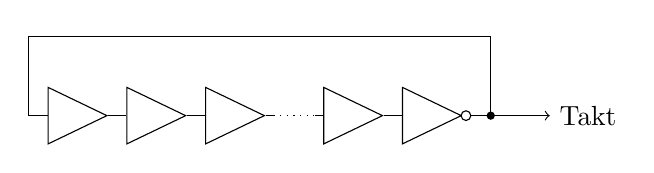
\begin{tikzpicture}[circuit logic US]
				\tikzstyle{branch}=[fill,shape=circle,minimum size=3pt,inner sep=0pt]

				\coordinate (ports) at (-2,0);

				\node [buffer gate] (b1) at (1,0) {};
				\node [buffer gate] (b2) at (2,0) {};
				\node [buffer gate] (b3) at (3,0) {};

				\node [buffer gate] (b4) at (4.5,0) {};

				\node [not gate] (n1) at (5.5,0) {};

				\draw (n1.output) -- ([xshift=7]n1.output) node[branch] (branch1) {}
				-- +(0,1) node (t1) {};

				\draw (b1.input) -- ([xshift=-7]b1.input) |- (t1.center);

				\draw (b1.output) -- (b2.input);
				\draw (b2.output) -- (b3.input);

				\draw (b3.output) -- ($(b3.output) + (0.1,0)$);
				\draw[dotted] ($(b3.output) + (0.1,0)$) -- ($(b4.input) + (-0.1,0)$);
				\draw ($(b4.input) + (-0.1,0)$) -- (b4.input);

				\draw (b4.output) -- (n1.input);

				\draw[->] (branch1.center) -- +(0.75,0) node [anchor=west] {Takt};


			\end{tikzpicture}
		\end{center}

		\begin{itemize}
			\item Die Frequenz des erzeugten Taktes ist nur durch die Laufzeit
				einer langen Kette von Gattern bestimmt.
		\end{itemize}
	\end{block}
\end{frame}

\liveDemo{Wir bauen einen ``Ringoszillator''}

\begin{frame}
	\frametitle{Wir bauen einen ``Ringoszillator'' --- Erkenntnisse}

	\begin{block}{Wir haben gesehen dass:}
		\begin{itemize}
			\item \ldots die Frequenz des Ringoszillators temperaturabhängig ist!
			\item Also muss auch die Gatterlaufzeit temperaturabhängig sein!
			\item Eine konstante Taktperiode ist also wieder eine
				Abstraktion.
		\end{itemize}
	\end{block}

	\begin{block}{Warum brauchen wir diese Abstraktion?}<2->
		\begin{itemize}
			\item Die Signallaufzeiten am Chip sind abhängig von Temperatur und Spannung.
			\item Darum will sich ein Programmierer nicht kümmern müssen,
			\item daher werden diese Abhängigkeiten verborgen:
			\item Wir wählen eine konstante Taktperiode, die größer ist als die Laufzeit unter
				den schlechtesten Bedingungen.
		\end{itemize}
	\end{block}
\end{frame}

\begin{frame}
	\frametitle{Grenzen der Chiptechnologie}

	\begin{alertblock}{Aber:}
		\begin{itemize}
			\item Woher kommen diese Laufzeiten eigentlich?
			\item Sind elektrische Signale nicht unendlich schnell?
		\end{itemize}
	\end{alertblock}

\end{frame}

\begin{frame}

	\begin{block}{Grenze 1: Lichtgeschwindigkeit \phantom{/}}

		\begin{itemize}
			\item $\SI{30}{\giga\hertz} =$ \num{30e9} Taktperioden pro
				Sekunde,
			\item Lichtgeschwindigkeit 	$c_0 \approx
				\SI{3e8}{\meter\per\second}$ (im Vakuum)\\
				Signale breiten sich am Chip mit $\approx \mathsf{^2/_3}~c_0$ aus.
			\item<2-> \alert<2>{In einer Taktperiode legt das Licht also nur
					\SI{1}{\centi\meter} zurück!}
				\item<3-> Bei einem Chip mit \SI{2}{\centi\meter} Kantenlänge
					braucht das Taktsignal also mehr als 2 Takte quer durch
					den Chip.
				\item<3-> Das widerspricht der Abstraktion, dass Taktflanken
					überall am Chip ``synchron'' stattfinden.
			\end{itemize}
		\end{block}

\end{frame}



\begin{frame}

	\begin{block}{Grenze 2: Lade-/Entladevorgänge}

		\begin{itemize}
			\item Gatter sind aus Transistoren aufgebaut.
			\item Idealerweise sind Transistoren Schalter (Abstraktion \ldots)
			\item Bei genauerer Betrachtung verhalten sich Transistoren (und
				Leitungen) wie Kondensatoren und Widerstände.
			\item Laden bzw.\ Entladen von Kondensatoren über einen Widerstand
				benötigt Zeit (vgl.: über Schlauch Gefäß füllen).
				% Publikumsfrage: Warum nimmt man nicht einfach einen dickeren
				% Schlauch?
			\item Diese Zeit begrenzt die erreichbare Geschwindigkeit des
				Chips.
		\end{itemize}
	\end{block}
\end{frame}


%\begin{frame}
%
%	\begin{block}{Grenze 2: Lichtgeschwindigkeit}
%
%	\begin{itemize}
%		\item $\SI{30}{\giga\hertz} = \SI{30e9}{\per\second}$,\\
%			$c \approx \SI{3e8}{\meter\per\second}$,\\
%			Chip: ca. $\SI{1}{\centi\meter\squared}$
%		\item \num{30e9} Mal pro Sekunde \SI{1}{\centi\meter} zurücklegen:
%			$\num{30e9} \cdot \SI{1}{\centi\meter\per\second} =
%			\SI{3e8}{\meter\per\second} = c$
%		\item D.h.\ in einem \SI{30}{\giga\hertz} Prozessor müssten sich die
%			Signale im Prozessor mit Lichtgeschwindigkeit ausbreiten.
%	\end{itemize}
%\end{block}
%
%\end{frame}


%\begin{frame}
%
%	\begin{block}{Problem 3: Ladungsausbreitung}
%		\begin{itemize}
%			\item Die Bewegung/Diffusion der Ladungsträger im Prozessor ist beschränkt
%			\item Bei Silizium typischerweise mit \SI{\approx
%				0.1}{\milli\meter\per\nano\second}
%		\end{itemize}
%	\end{block}
%
%\end{frame}
%


\begin{frame}

	\begin{alertblock}{Mehr Rechenleistung bei gleicher Geschwindigkeit?}
		Kann man die Physik überlisten?
	\end{alertblock}

\end{frame}

\begin{frame}

	\begin{block}{Lösung 1: Multi-Core und vernetzte Rechner}
		\begin{itemize}
			\item Moderne Desktop Computer: \numrange{4}{16} Prozessoren
				(Cores) verbaut in einem Chip, Tendenz steigend.
			\item Moderne Grafikkarten: über 1000 ``Cores''.
			\item Parallele Programme erfordern neue Programmiertechniken; \\
				\alert{große Herausforderung für die Informatik!}
		\end{itemize}
	\end{block}

\end{frame}

\begin{frame}

	\begin{block}{Lösung 2: Spezialisiertes Design}
		\begin{itemize}
			\item Bisher betrachtet: ``general-purpose'' Prozessoren die für
				verschiedenste Einsatzbereiche geeignet sind.
			\item Programmierbarkeit und Vielseitigkeit kosten Effizienz.
			\item Spezialisierte Designs (ASICs) erreichen eine Effizienz die
				mit general-purpose Lösungen nicht erreichbar ist.
			\item Höherer Entwicklungsaufwand, aber unverzichtbar für
				Anwendungsbereiche, in denen general-purpose Lösungen die
				benötigten Anforderungen (Performance, Verlustleistung,
				Fehlertoleranz, \ldots) nicht erfüllen.
		\end{itemize}
	\end{block}

\end{frame}


	\include{studienplanTI}

	
\begin{frame}
	\frametitle{Zusammenfassung}

	\begin{block}{Wir haben erlebt, dass \ldots}
		\begin{itemize}
			\item Abstraktion ein mächtiges Werkzeug ist,
			\item dessen Grenzen man allerdings stets genau kennen sollte.
			\item Diese Kompetenz vermittelt ein Studium.
			\item Erlernen von Grundlagen ist essenziell
			\item \ldots und macht Spaß!
		\end{itemize}
	\end{block}
\end{frame}

%\begin{frame}
%	\frametitle{Ein Ausblick auf morgen}
%
%	\begin{block}{Wie funktioniert eigentlich ein Computer?}
%		\begin{itemize}
%			\item Abstraktionsebenen im Computer.
%			\item Vom Befehl zum Schalten des Transistors.
%			\item Auch hier zahlt sich Hintergrundwissen aus!
%		\end{itemize}
%	\end{block}
%\end{frame}

\end{document}
